\documentclass{article}[11pt]
\usepackage{graphicx}
\usepackage{tabularx}
\usepackage{natbib}


\usepackage{array}
\usepackage{amsmath}
%\usepackage[backend=bibtex]{biblatex}
\bibliographystyle{..//refs/styles/besjournals.bst}
\setkeys{Gin}{width=0.8\textwidth}
%\setlength{\captionmargin}{30pt}
\setlength{\abovecaptionskip}{10pt}
\setlength{\belowcaptionskip}{10pt}
 \topmargin -1.5cm 
 \oddsidemargin -0.04cm 
 \evensidemargin -0.04cm 
 \textwidth 16.59cm
 \textheight 21.94cm 
 \parskip 7.2pt 
\renewcommand{\baselinestretch}{1.2} 	
\parindent 0pt
\usepackage{lineo}
\linenumbers
%\usepackage{xr}
\usepackage{xr-hyper}
\usepackage{hyperref}
\externaldocument{SUPPinvasive}

\title{Seedling competition between two native %Honewort (\textit{Cryptotaenia canadensis}) 
and invasive %Dame's Rocket (\textit{Hesperis matronalis}) 
woodland herb species is mediated by relative germination timing}

\author{D.M. Buonaiuto $^{1,2,a}$, E.M. Wolkovich$^{3}$}

\usepackage{Sweave}
\begin{document}
\input{invasive-concordance}
\maketitle
\noindent \emph{Author affiliations:}\\
\noindent $^1$Arnold Arboretum of Harvard University, Boston, Massachusetts, USA. ORCID: 0000-0003-4022-2591\\
$^2$Department of Organismic and Evolutionary Biology, Harvard University, Cambridge, Massachusetts, USA \\
$^3$Forest \& Conservation Sciences, Faculty of Forestry, University of British Columbia, Vancouver, British Columbia, Canada\\
$^a$Corresponding author: 617.823.0687; dbuonaiuto@g.harvard.edu\\
\pagebreak
\section*{Abstract}
Invasive plant species are often characterized by rapid germination and precocious phenology. Theory suggests that early germination may provide invaders with significant competitive advantage over slower germinating natives, but the relative contribution of rapid germination vs. other intrinsic competitive traits to the success of plant invaders is poorly characterized. Depending on the relationship between germination timing and competition, alterations to patterns of germination phenology due to anthropogenic climate change may either increase the dominance of invaders or buffer native communities against their impacts. Predicting invasion dynamics and the structure and function of plant communities of the future will require clarifying the relationship between climate variability, phenological differences among species and competitive outcomes.

To fill this gap, we performed a sequence of controlled environment experiments. First, we evaluated how variation in cold stratification duration and growing temperatures impacted the relative germination phenology of eleven temperature herbaceous species. We then leveraged these differences to indirectly manipulate the relative germination phenology of two species, the invasive \textit{Hesperis matronalis} and native \textit{Cryptotaenia canadensis}, planted in competition, in order to quantify the effects of their phenological differences on competitive outcomes.

We found that precocious germination phenology roughly doubled the competitive impact of \textit{H. matronalis} relative to it's intrinsic competitive traits, and that phenological advances of just two-three days relative to \textit{C. canadensis} were enough to secure its competitive dominance at the seedling stage. We also found that the germination phenology of most native species in our study was strongly associated with cold stratification duration, suggesting that decreases in cold stratification conditions due to anthropogenic global warming will likely increase the phenological advantage of rapidly germinating invaders. 

Add a sentence here. Our results suggest the phenological diversity may be an important factor for maintaining native plant communities into the future. %289 words


\section*{Introduction}
 A central tenet of community assembly theory is that the order of arrival of species to a community mediates inter-specific interactions and can dictate the trajectory of community structure in the long term \citep{Fukami2015}. These historical contingencies, known as priority effects, have been shown to alter the structure and function of communities, driving communities to long-term alternate stable states \citep{Fukami2011}. Yet in many ecosystems, plant communities must re-assemble each year after a period of dormancy. In these communities, priority effects are the products of phenology, the timing of seasonal life cycle events,% and the rate at which dormant plants and seeds respond to their environment and resume growth or germinate when favorable conditions return 
rather than the timing of the arrival of propagules, which in many cases occurs prior to the dormant season \citep{Rudolf:2019aa,Howe:1982aa,Baskin:1988aa}. 
%These seasonal, or short-term priority effects \citep{Wainwright_2011,Young:2017aa}, may be important mediators of plant interactions, and have been invoked to explain the competitive dominance of some species (when strong competitors also have rapid/early germination) \citep{Gioria2018}, and inter-specific coexistence (when weaker competitors have rapid/early germination and/or priority varies over time) \citep{Towers:2020aa}.

Invasive plants are often characterized by rapid germination and precocious phenology under a wide variety of environmental condition \citep{Gioria2018,Gioria:2017wo,Wolkovich:2011uh,Smith:2013uj}. By contrast, native plants tend to exhibit more constrained germination cues \citep{Marushia:2010ug}. In many temperate systems, seeds of native plants are dispersed with deep physiological dormancy, requiring prolonged exposure to specific environmental conditions, such as cold stratification (cool temperatures 0-10$^{\circ}$ C) to break dormancy and stimulate germination \citep{Brink:2013wr,Cavieres:2017aa,Bradford:2007tj}.

These differences in germination physiology can yield strong differences in the relative germination phenology of invasive and native plants, with invaders germinating well before their native competitors \citep{Gioria:2017wo}. We refer to this difference in relative germination timing among species as \textbf{phenological advantage}. Phenological advantage can contribute significantly to the competitive abilities, and ultimately invasion success, of invasive plants by allowing them to begin drawing down seasonal resources and modifying their environment before their native competitors emerge \citep{Kardol2013}. We refer to this effect of phenological advantage on interspecific competition as a \textbf{seasonal priority effect} \citep{Wainwright_2011}.

Yet, it is difficult to quantify the overall contribution of seasonal priority effects to the competitive success of invaders. Germination is notorious difficult to monitor in the field, and rapid phenology often co-varies with other competitive traits \citep{Dickson2012,Milbau:2003vt,HAO:2009vh}. % such as high fecundity, growth rates, and stress tolerance 
One way that this problem has been addressed is through experiments that vary phenological advantage by sowing competing seeds at different time intervals \citep{Young:2017aa}. While these experiments have provided strong evidence that phenological advantage on the order of just days to weeks can yield substantial priority effects \citep{Weidlich:2020aa}, the highly artificial experimental set-up is difficult to translate into natural communities in which priority effects would be mediated by climate. As such, the relative importance of phenological advantage vs. other competitive traits to invasion success and competition dynamics in nature remains poorly characterized. % probably need to make this less picante

Understanding the role that phenological advantage plays in mediating the dynamics of interspecific competition is critical for predicting and managing the structure and function of plant communities in the face of anthropogenic climate change. Due  to interspecific differences in germination responses to environmental variation, sustained alterations to environmental conditions are already shifting community-wide patterns of germination \citep{Walck2011}. If patterns of germination are indeed tightly link the the competitive dynamics of communities than phenological re-organization is likely to shift the strength of species' interactions, change patterns of invasion, and strongly influence biological filtering of plant communities. 

In this study, we leveraged among-species differences in germination phenological sensitivity to environmental variation in order generate contrasting levels of phenological advantage among competing species. This approach allowed us to assess the maximum variation in phenological advantage due to climate variation among co-occurring species and quantify the contribution of seasonal priority effects to the competitive outcomes of interacting species. First, we performed a series of germination assays in controlled environments under varying temperature regimes to estimate a realistic range of climate-driven variation in phenological advantage for a suite of widespread invasive and native forbs.  We then performed competition trials for two focal species (the North American invasive \textit{Hesperis matronalis} and native \textit{Cryptotaenia canadensis}) under contrasting environmental conditions to indirectly manipulate the phenological advantage between them and quantify the contribution of seasonal priority effect to their competitive dynamics.

Through opporationalizing unique species-level responses to environmental change, our experiments constrain the magnitude of variation in phenological advantage to biological realistic scenarios. This allow us to robustly estimate seasonal priority effects on plant competition in a way that is more readily translatable field conditions, and assess to what degree seasonal priority effects mechanistically contribute to the competitive success of invasive species. Through linking climate variation, phenological advantage and seasonal priority effects, our study has important implications for how anthropogenic climate change will alter phenological assembly and, in turn, plant community interactions in the decades to come.
% Compete them to assess the influences of priority effect on competitive outcome and quantify SPE's contribution vs. other intrinsic competition traits.
%Yet the differential sensitivity to the environmental cues that is driving shifts in community patterns of phenology can also be leveraged to evaluate the role of seasonal priority effect is inter-specific competition. Because germination conditions vary among years, that germination responses between competing species will converge and diverge periodically over time, depending the their specific sensitives and the climate they experience. This variation can be leverage for mechanistic tests of SPEs by quantifying how the phenological lag between species changes under realistic climate variation and the effect of this variation on competition.
%In ecological systems where dormancy release is controlled by temperature, cohabiting species respond with different sensitivities to these elements; and this is be especially true for invasive species which evolved under different climate condition in their home vs. invaded ranges \citep{}.
%\item And climate elements vary over time
%\item Together, this suggests that germination or phenological responses between competing species will converge and divirge periodically over time, depending the their specific sensitives and the climate they experience.
%\item This variation can be leverage for mechanistic tests of SPEs by a) qunatify how the phenoligical lag between species changes under realistic climate variation , and b) the effect of this variation on competition
%\section{Introduction}
%\textbf{A core task of invasion biology it to identify trait that make a species likely do be invasive}
%\begin{enumerate}
%\item Invasive species are characterized by rapid germination and precocious phenology
%\item Being so early may function as a seasonal priority effect-niche premption and such
%\item This seasonal priority effect might contribute to the competitive dominacne and invasion success of invasives
%\end{enumerate}
%\textbf{But it is difficult to infer mechanism from observational studies}
%\begin{enumerate}
%\item Because rapid phenology often covaries with other competitive traits. You'd need super high resolution phenolgy and %climate data.
%\end{enumerate}

%\textbf{Experiments can test role of SPE's in plant competition}
%\begin{enumerate}
%\item  A common approach is to use sequential planting studies.
%\item recent review paper on these experiments by \citet{Weidlich:2020aa}: 42\% of such studies included planting interval treatments of less than 1 month, approximating the time scale of SPEs and all found evidence of priority effects. (How many were invasive vs. native?)
%\end{enumerate}

%\textbf{Yet the extent to which these studies are generailizable is questionable}
%\begin{enumerate}
%\item  Almost all mechanistic tests for SPEs to date have been performed using species from temperate grasslands \citep{Weidlich:2020aa}, whose germination behavior may differ substantially from taxa in other habitats \citep{Tudela-Isanta:2018aa}.
%\item In many ecosystems, plant communities must re-assemble each year after a period of dormancy. In these communities, priority effects are largely the product of the rate at which dormant plants and seeds respond to their environment and resume growth or germinate when favorable conditions return \citep{Rudolf:2019aa}, rather than the the timing of the arrival of propagules, which in many cases occurs prior to the dormant season \citep{Howe:1982aa,Baskin:1988aa}.
%\item Therefore, sequential plantings cannot address how important SPE's are in nature because the priority effect is 100\% contigent on the choice of the treatment.
%\%end{enumerate}
%\textbf{In ecological systems where dormancy is common like temperate  and boreal forest, say a few other here, environmental conditions such as temperature (cold stratification and incubate), soil moisture, and light control the release of dormancy and germination or growth.}
%\begin{enumerate}
%\item Cohabiting species respond with different sensitivites to these elements; and this may be especially true for invasive species which evolved under different climate condition in their home vs. invaded ranges.
%\item And climate elements vary over time
%\item Together, this suggests that germination or phenological responses between competing species will converge and divirge periodically over time, depending the their specific sensitives and the climate they experience.
%\item This variation can be leverage for mechanistic tests of SPEs by a) qunatify how the phenoligical lag between species changes under realistic climate variation , and b) the effect of this variation on competition
%\end{enumerate}
%\textbf{Leveraging natural climate variation to test SPEs has major beneifits}
%\begin{enumerate}
%\item SPE's are a cornerstone of community assembly theory and modern coexistence theory, and mechanistically qunatifying their contribtion in community interactions is important
%\item Anthropogenic climatic change is altering the  environments \citep{Walck2011} and changing  germination and phenology patterns. Such sustained alterations to environmental cues have potential to disrupt SPEs, shifting balances of species' interactions, changing patterns of invasion, and strongly influence biological filtering of communities..
%\item So assessing the role of SPE's in species interactions under more realistic germination environments is timely because it can be used to improve spatio-temporal predictions of species interaction under novel climate conditions.
%\end{enumerate}%
%
%\textbf{While invasibility, competion, coexistance etc is a property of individual and community interactions, pair-wise comparisons have been a useful tool to identifying and quatify mechanisms of species interactions}
%\begin{enumerate}
%\item Why am I saying this? Probably to justify the limited taxonomic scope of my study
%\end{enumerate}
%
%\textbf{Using a combination of germination assays, competition trials and climate projections, we:}
%\begin{enumerate}
%\item Quantify gernmination behavior of varying environments to estimate a realistic range of climate driven priority between an widespread invasive and native forb species. 
%\item Compete them to assess the influences of priority effect on competitive outcome and quantify SPE's contribution vs. %other intrinsic competition traits.
%\item Use relationship between climate and germination behavior to make first-pass, quick and dirtay and rough prediction about where where interactions between these two species may shift with climate change as a proof-of-concept case study to build on in the future.
%\end{enumerate}
\section*{Methods}
\subsection*{Focal species}
 Dames Rocket (\textit{Hesperis matronalis}) is a herbaceous biennial/perennial species in the \textit{Brasicaeceae} family, originally from Eurasia, and introduced to North America in the 19th century \citep{Francis:2009wz}. It  can rapidly invade  meadows, forest edges and woodlands, forming thick stands and excluding native vegetation \citep{Francis:2009wz}. It is currently listed as a noxious or invasive weed is several states and provinces in the United States and Canada \citep{Susko:2008ut}. Honewort (\textit{Cryptotania canadensis}) is a herbaceous perennial in the \textit{Apiaceae} family, native to forests and woodlands of eastern North America \citep{Hawkins:2007vb}. The  habitat overlap of these two species suggests that they may compete in nature. While their habitat requirements may be similar, the two species display a substantial different germination niche, making them a suitable model for our study. \textit{C. canadensis} seeds are classified with deep physiological dormancy and require a substantial period of cold moist stratification to release dormancy and initiate germination \citep{Baskin:1988um}. While some reports suggests that cold stratification enhances germination in \textit{H. matronalis} at low incubation temperatures, several studies have demonstrated that fresh and after-ripened (dry-stored) seeds of \textit{H. matronalis} are capable of rapid and complete germination at a wide range of temperatures \citep{Susko:2008ut}. These contrasting germination dynamics among species suggest that phenological advantage between them is likely to be strong mediated by cold stratification and incubation variation.  

\subsection*{Germination Assays}
To investigate the relationship between environmental variation and relative germination timing between competing species, we obtained seeds of 14 spring-germinating herbaceous species common to temperate forest-edges, including our focal species  \textit{C. canadensis} and \textit{H. matronalis}, from domestic plant nurseries (see Tab. \ref{tab:specs} for details). We performed germination assays in the growth facilities of Arnold Arboretum in Boston MA (42.3074$^{\circ}$ N, 71.1208$^{\circ}$ W). We assigned seeds to a fully crossed set of twenty experimental treatments; 10 levels of of cold stratification duration (0,2,4,5,6,7,8,9,11,13 weeks at 4$^{\circ}$ C) and two levels of incubation temperature (warm--- 25$^{\circ}$ C:15$^{\circ}$ C (day/night), cool--- 20$^{\circ}$ C:10$^{\circ}$ C (day/night)).

\noindent  Prior to applying experimental treatments we performed a ``float test" in which all seeds were placed in distilled water, and unfilled seeds (floating) were removed from the experiment \citep{Baskin2014}. We imbibed the remaining seeds in distilled water for 24 hours and then placed 20 seeds per species/ treatment combination in petri dishes on moist pool-filter sand. We replicated each treatment combination three times. For the cold stratification treatments, we wrapped petri dishes in aluminum foil to prevent light exposure and placed them in a growth chamber at 4$^{\circ}$C. After each stratification interval, we transferred the petri dishes to their assigned incubation chamber for 25 days, moistening the germination substrate as necessary to maintain maximum saturation of the medium without flooding the seeds. We check for new germinates every 2 days, defining a seed as germinated when its radical or cotyledon tissue was visible \citep{Baskin2014}. We assessed the viability of any seeds that did not germinate in the 25 day incubation period by performing a ``crush test" in which we applied pressure to the intact seed to evaluate its condition \citep{Baskin2014}. We excluded any seeds deemed unviable from all subsequent analyses. Due to the staggering of our stratification treatments the experiment took place between 27 August- 12 December 2018.\\

\subsubsection*{Statistical analysis}
To assess inter-specific differences in the relationship between germination rate and temperature variability, we fit a Bayesian mixed-effect accelerated failure time model (AFT) with weeks of stratification and incubation temperature as fixed effects and species as a random effect. Three species, (\textit{Carex grisea}, \textit{Impatiens capendsis} and \textit{Phlox cuspidata}), did not germinate at high enough fractions in our assays to analyze, so our final analysis consisted of 11 species.\\ 

We chose an AFT model as it allowed for us to account for viable seeds that did not germinate during our incubation window, letting us robustly compare germination timing (t50 or time to 50\% germination) even among treatments with different final germination percentages in the time frame of the experiment \citep{Soltani:2015aa}. One drawback of this approach is that this class of models assume that all viable seeds will eventually germinate, which we would not expect to be true in nature. For this reason, we considered any estimated t50 values greater than 40 days to indicate that seeds would not reach 50\% germination under those conditions. \\ 

In addition to our full species model described above, we fit an additional AFT model on a subset of data including only \textit{C. canadensis} and \textit{H. matronalis} in order to obtain higher resolution estimates for the germination dynamics for our two focal species. In this model we included species as a fixed effect in addition to incubation temperature and stratification duration. 

\noindent We fit the models using the R package ``brms" \citep{Burkner2018} using a weibull distribution for the model's likelihood function. We ran the model on four chains with 4000 iterations and a 3000 iteration warm up for a total of 4000 posterior draws for each parameter using weakly informative priors. We assessed  model performance through ensuring $\hat{R}$s were between 1 and 1.01 and bulk and tail effective sample sizes were high.

\subsection*{Competition Trials}
%To quantify the contribution of seasonal priorty effects to inter-specific competition dynamics, we chose two species from our germination trial \textit{Cryptotaenia canadensis} and \textit{Hesperis matronalis} for competition trials. We chose these species because the germination of \textit{C. candensis} advanced strongly with increasing cold stratification, while seeds of \textit{H. matronalis} germinated rapidly under all conditions suggesting that under low stratification treatments there would be a strong priority effect between the species that would diminish as stratification time increased. Additionally \texit{H. matronilis},originally from Eurasia, is considered an invasive species or noxious weed in many parts of North America and so evaluating the role of SPE's in this species's competitive ability has potential applied benefits for the management of this species.\\
\noindent To quantify the contribution of seasonal priority effects to inter-specific competition dynamics of our focal species we performed competition trials under controlled condition in a research greenhouse at the Arnold Arboretum from October 2020-February 2021. We planted seeds of \textit{C. canadensis} and \textit{H. matronalis} into 3.5 inch square pots, employing a response surface design where we varied both the overall density of seeds and proportion of each species in each pot \citep{Inouye2001}. High and low density treatments consisted of 14 and 8 seeds total seeds respectively. Our proportion treatments (100:0\%. 25:75\%, 50:50\%, 75:25\%, 0:100\% (species A :species B)) Each density by proportion treatment was replicated six times. %This design allows us to evaluate effects of inter- and intra- specific competition and density dependence independently and in association with our experimental treatment.\\

\noindent We randomly assigned half of the pots low (45 days) and high (72 days) cold stratification treatments at 4$^{\circ}$ C. We staggered the start of the treatments, so that at the conclusion of the pre-treatment, all pots were transferred to a heated greenhouse maintained at 15-25$^{\circ}$C with 14 hours of supplemental light. Germination was observed daily from 24 December 2020 - 13 January 2021 and every two days from 15 January 2021 to 01 February 2021. The locations of each pot in the greenhouse were randomly reassigned every three days to minimize any blocking effects on germination or growth.

\noident After 35 days, we added 1 tsp per 1 gallon of water of Peter’s 20-10-20 liquid feed fertilizer to all pots. After 62 days, we harvested the above-ground biomass from all pots, dried it in a oven for 48 hours at 60$^{\circ}$C, and recorded the dry weight of each species/pot using a Mettler balance.\\

\subsubsection*{Statiscal analysis}
\noindent We quantified the phenological advantage between the species by subtracting the mean germination time (MGT) of \textit{H. matronalis} from that of \textit{C. canadensis} in each pot. This allowed us to evaluate the effect phenological advantage with a regression design \citep{Cottingham:2005ud}, with advantage values ranging from -1.3 to 9.5 (\textit{C. candensis} mean germination time 1.3 days earlier to 9.5 days later than that of \textit{matronalis}).

For each plot, we calculated the relative growth rate difference among species using the equation below modified from \citet{Connolly2005}.
\begin{align*}

RGRD &= $ ln(\frac{Y_{Cc}}{y_{Cc}}) &- ln(\frac{Y_{Hm}}{y_{Hm}}) $
%ln({Y}\frac{y})\ %- ln(\fract{Y_{Hm}}{y_{Hm}})

\end{align*}

where $Y_{Hm}$ and $Y_{Cc}$ are the final biomass of the species at the end of the experiment and $y_{Hm}$ and $y_{Cc}$ are the initial biomass of the seeds planted at the outset of the experiment. For this calculation we obtained estimates of seed mass for our focal species from the Kew Gardens Seed Information Database \citep{}.  

We then modeled the effect of seedling density of \textit{C. canadensis}, \textit{H. matronalis} and phenological advantage using Bayesian linear regression  using the R packages ``brms'' \citep{Burkner2018}. Using weakly informative priors, we ran this model on 4 chains, with 4000 iterations per chain and a warm up of 3000 iterations, for a total of 4,000 posterior samples per parameter. The model is written below:

\begin{align*}

RGRD &= \alpha + \beta_{1}y_{Hm} + \beta_{2}y_{Cc} + \beta_{3}MGT + \epsilon

\end{align*}

where  $\beta_{1}$ and $\beta_{2}$ are the known as the species influence parameters, or the estimated effect of increasing the seedling density of each species by one individual on the RGRD \citep{Connolly2005}, and $\beta_{3}$ is the priority effect, or the effect of increasing the difference in MGT between  \textit{H.matronalis} and \texti{C. canadensis}. In this formulation, $\alpha$ is an un-interpretable intercept \citep{Connolly2005}.


To assess whether the rapid germination phenology of \textit{H. matronalis} modified the germination niche of \textit{C. canadnesis} we performed two additional Bayesian  regression analyses. We assessed the influence of planting type (single species vs. mixed competition) on the the likelihood of \textit{C. canadensis} germination using a Bernoulli distribution and the mean germination time of \textit{C. canadensis} using a Gaussian distribution. In both models we included stratification treatment as a fixed-effect co-variate. As above, we ran these models using the R packages ``brms''\citep{Burkner2018},  with weakly informative priors.

%\subsection*{Focal species}
%\subsection*{Germination Assays}
%\subsection*{Competition Trials}
%\subsection*{Data analysis}
%\textbf{Some thoughts on Connolleys RGRD models}
%\begin{enumerate}
%\item Data at the plot level which makes large assays like the one I did tractable compared with spatially explict ones like heygi index or neighborhood
%\item Also is desinged for signle season dynamics unlike Lotke-Volterra and the usual
%\item Weakness, isn't designed for monoculture treatments( which we explictely put in out study ) since you an't have the log of zero. Maybe I overcome this by %converting 0s to 00000.1

%\end{enumerate}
\section*{Results}
\subsection*{Germination advantage}
Across all species in our germination assays, the time to 50\% germination advanced by 6.14 days per week of cold stratification (converted from log scale; mean: -0.14, $CI_{90}:$\textit{-0.20, -0.08}), though the strength of this effect varied significantly among species  (Fig. \ref{fig:musurv}a, Fig. \ref{fig:AFTall}). The overall estimated effect of incubation temperature on germination phenology was weak, delaying time to 50\% germination by 1.45 days per  $^{\circ}$C (converted from log scale; mean: 0.03, $CI_{90}:$\textit{-0.04, 0.10}) but this was due to strong inter-specific differences in the directional response to increasing incubation temperatures. The germination phenology of 5 species advanced with increasing incubation temperatures, and was delayed for 6 species (Fig. \ref{fig:musurv}b).\\%  suggesting that for these species, our warm incubation treatment exceeded their thermal optimum.\\

Considering our focal species, \textit{H. matronalis} reached 50\% germination in under five days for all environmental treatments, always exceeding 75\% germination regardless of environmental conditions (Fig. \ref{fig:aft}, Tab. \ref{tab:germcomps}). Increasing cold stratification duration and incubation temperature only marginally only enhanced the germination rate of this species (Fig. \ref{fig:aft}). By contrast, increasing incubation temperature had a delaying effect of the germination rate of \textit{C. canadensis}, suggesting that the mean 20$^{\circ}$C temperatures of our warm incubation treatment are supra-optimal for the species (Fig. \ref{fig:aft}). Without sufficient cold stratification ($>$7 weeks for low incubation and $>$ 10 weeks for high incubation temperatures), seeds of  \textit{C. canadensis} did not reach 50\% germination during the duration of our experiment (Fig. \ref{fig:aft}, Tab. \ref{tab:germcomps}). However, under high levels of cold stratification germination rates of \textit{C.canadensis} began to converge on those of \textit{H. matronialis}, and at levels of stratification greater than 10-12 weeks and low incubation temperatures, the germination rate and fraction of \textit{C.canadensis} was well matched to that of \textit{H. matronalis} (Fig. \ref{fig:aft}, Tab. \ref{tab:germcomps}).

Given the strong inter-specific differences in phenological sensitivity to stratification and incubation, our results indicate that climate strongly shapes patterns of phenological assembly, and patterns of phenological advantage can be highly variable due to climate variation.

\subsection*{Germination priority effects}
In the absence of phenological advantage, the influence of adding one individual of \texit{H. matronalis} was almost 4x less than adding one individual of \texit{C. canadensis} to the plot-level RGRD (species influence parameters:  \textit{H. matronalis}: 0.126, $CI_{90}$: \textit{0.08,0.17},\textit{C. canadensis}: -0.40, $CI_{90}$: \textit{-0.46, -0.35}). Every day increase in the phenological advantage of \textit{ H. matronalis} had approximately the same influence on shifting the community biomass composition towards \textit{H. matronalis} as adding an individual of that species to the community (priority effect: 0.146, $CI_{90}$: \textit{0.09, 0.20},Fig. \ref{fig:RGRD}, Tab. \ref{tab:RGRD}). Together, these result suggest that \textit{H. matronalis} will come to dominate the community biomass composition unless \textit{C. canadensis} is at high relative abundance or the phenological advantage of \textit{H. matronalis} is small (Fig. \ref{fig:3D}).

\subsection*{Priority effects and germination niche modification}
We observed no evidence that the rapid germination of \textit{H. matronalis} adversely modified the germination niche of \textit{C. canadensis}. Neither the likelihood of germination nor the mean germination time of \textit{C. canadensis} were suppressed when the species grew in mixed species competition vs. single-species plots (Fig. \ref{fig:nichemod}). Rather, at low stratification levels, the presence of rapidly germination \textit{H. matronalis} might have positively affected the germination fraction of \textit{C. canadensis}, (Fig. \ref{fig:nichemod}a), though there is high uncertainty around this comparison.

\section*{Discussion}

\subsection*{Germination advantage as a seasonal priority effect} 
In this study, we found that climate driven differences in germination advantage was a key mediator of the competitive dynamics between our two focal species \textit{H. matronalis} and \textit{C. canadensis}. In the absence of phenological advantage, the species influence parameter estimates from our model (representing the intrinsic competitive abilities of seedlings of each species) suggest that \textit{C. canadensis} is the stronger competitor (Fig. \ref{fig:RGRD}, the influence parameter of \textit{C. canadensis} is significantly more negative than that of \textit{H. matronalis} is positive ). However, the influence of one day of phenological advantage for \textit{H. matronalis} virtually doubled the influence of this species on the final community composition, suggesting that seasonal priority effects play a major in the competitive success of \textit{H. matronalis} (Fig. \ref{fig:RGRD}). Using the species influence parameters and priority effect we estimated in our model we determined that \textit{C. canadensis} can compete with the invasive \textit{H. matronalis}, but only at high relative abundance levels and when phenological advantage is low (Fig. \ref{fig:3D}). While it is certainly possible that \textit{H. matronalis} might interact differently with other species, the results of our pair-wise competition trials suggest that both seasonal priority effects manifested through rapid germination phenology and propagule pressure are mechanistically related to the competitive dominance, and ultimately invasion success of \textit{H. matronalis}.

While we found that seasonal priority effects strongly impacted competition among seedlings, our experiment was not able to quantify the role of seasonal priority effects in influencing the long-term, among year dynamics of these perennial species, which may be quite different from within-season seedling interactions \citep{}. Many studies suggest that these short term priority effects many be transient, though several studies that used staggered planting methods at similar scale to the phenological lags we observed in our trials saw the influence of these initial priority effect on community composition several seasons later \citep{Weidlich:2020aa}.  In perennial communities, these long terms dynamics are even more difficult to assess as many perennial herbs, \textit{C. canadensis} included, rely heavily on vegetative reproduction \citep{Hawkins:2005ve}. Because of this, the kind of seedling to seedling competition we observed in our experiment, may be less common, and therefore less important to overall community demography than competition among vegetative ramets, or between ramets and seeds \citep{}. Understanding how phenological differences across life stages of of long-lived perennial plants affects within season competition is an important next step for predicting how communities may be impacted by climate change.

Our competition trials did not suggest any evidence that the rapid germination phenology of \textit{H. matronalis} impacted the germination niche of \textit{C. canadensis} in any regard (Fig. \ref{fig:nichemod}). This indicates that the mechanism underlying the seasonal priority effect if \textit{H. matronalis} is likely niche preemption, though we can not rule out the possibility that niche modification occurs at the seeding stage as well. % could talk about how this contrast with alleleopathy of other forest invaders like garlic mustard.

\subsection*{Environmental drivers of seasonal priority effect}
Our results join a growing body of experiments demonstrating that relative germination phenology can function as a seasonal priority effect, enhancing the performance of the earliest germinating species at the expense of later germinants \citep{Korner2008,Dickson2012,Ross1972}. While this effect has been primarily commonly demonstrated in experiments in which the planting of competing seeds is staggered at increasing intervals \citep{Young:2017aa,Weidlich:2020aa}, our experimental results advance the understanding of the role of seasonal priority effects on competition by identifying a natural mechanism, species' differential sensitivity to climate, that can generate seasonal priority effects.

We found that climate variation, especially the duration of cold stratification was tightly linked to mediating the phenological advantage between \textit{H. matronalis} and \textit{C. canadensis}, and that small changes in advantage, of as few two days (Fig. \ref{fig:RGRD}). Interestingly, the difference in phenological advantage among our focal species was much higher in our germination assays than in our competition trials even at comparable levels of stratification. There are likely several explanations for these differences.

Perhaps the most important is that we used different metrics of germination speed, time to 50\% germination (t50) and mean germination time (MGT) in each experiment. While the metrics are related and often confused, there are important differences between them that make one or the other more appropriate for the two types of experiments we ran. The t50 is an estimate of the time to 50\% germination of all seeds planted, while MGT is a measure of the time to 50\% germination of only individuals that actually germinated \citep{Soltani:2015aa}. In comparative germination assays, t50 is a better metric because is standardized phenological estimates across variable germination fractions. In our competition trials it would not have made sense to account for the the germination speed of individuals that did not germinate, because only germinated individuals were influencing the competitive dynamics of our species. Because MGT is sensitive to the final germination fraction, it is not surprising the MGT measurements in the competition trials  were lower than the t50 estimates in the germination assays.

Additionally, the incubation temperatures in our greenhouse competition trials were more variable than in our growth chamber germination  assays. The lower germination fractions we observed in \textit{C. canadensis} under greenhouse conditions suggests that the temperature range was likely supra-optimal for this species, and the lower germination fraction increased the difference between t50 estimates and MGT measurements. Finally, germination assays and competition were conducted in different growth media (filter sand vs. potting soil), which have different moisture retention and light transmissible  capacities. Germination media can strongly affect germination rates \citep{}, which may further explain differences among our two experiments.

However, despite these differences, the relationships between cold stratification germination phenology and phenological advantage were robust across our experiments, with increased cold stratification strongly advancing the germination phenology of \textit{C. canadensis} and weakly that of \textit{H. matronalis}, resulting in weaker phenological advantage at higher stratification levels. (Fig. \ref{fig:aft},Fig. \ref{fig:MGTsup}).

\subsection*{Seasonal priority effects and anthropogenic climate change}
The implications for the role of climate variability in mediating seasonal priority effects is two fold. First, our results suggest that inter-annual climate variability should generate both among and within season variation in competition strength among species, potentially driving species coexistence via the storage effect \citep{}. Second, the key role we observed of climate in generating germination advantage and therefore seasonal priority effects suggests that sustained alteration to historic patterns of climate variability, like those driven by anthropogenic climate change, are likely to strongly alter the dynamics of competing seedlings which will have downstream effects on the structure and function of plant communities.

In our study,the priority advantage of \textit{H. matronalis} was maximized under lower stratification treatments and warmer incubation temperatures. This suggests that the warming temperatures associated with anthropogenic climate change may increase the magnitude of seasonal priority effects, largely due to the delay of germination in more climate sensitive native species like \textit{C. canadensis}.

Importantly, invaders invade plant communities, not single species populations, and while we were only able to quantify the impact of seasonal priority effects for two species, our multi-species germination assays allow us to make some inference about how patterns of germination advantage may shift at the community level. At low stratification duration, less climate sensitive invaders can exploit the early season germination niche with less competition from natives than at when stratification is higher. Projections based on our germination time models suggest, that under low stratification (6 weeks) that ratio of native to invasive species we studied that germinate well within the first 20 days of the climatic growing season is small (Fig. \ref{fig:comm}, 3:2 and 4:2 under cool (15$^{\circ}$C) and warm (20$^{\circ}$C) growing temperatures respectively), while under longer stratification duration (12 weeks), the ration is much higher (6:2 and 5:2 cool vs. warm) and the phenological advantage of the invaders significantly reduced (Fig. \ref{fig:comm}). While the conversion of phenological advantage into seasonal priority effects is likely species specific, the strong positive relationship between advantage and competitive impact we observed in our study suggests that the phenological advantage that comes with warmer conditions is likely to increase the impact of rapid germinating invaders through seasonal priority effects. 

One important caveat is that in our experiment, there was no cost to germinating too early. It is generally accepted that optimum germination phenology is driven by a trade-off between maximizing the growing season and the risk of exposure to damaging environmental episodes when germinating too early \citep{}. In dry grassland ecosystem, it has been demonstrated that the precocious germination of invasive has a substantial cost in water availability is too low \citep{Wainwright_2011}. In temperate forest ecosystems, the primary risk of early phenology is damage from late season frost \citep{}. Future work could further clarify the contribution of seasonal priority effects to community interactions by experimentally manipulating this trade-off as well.

Because we found that seasonal priority effects strongly mediated competition for at least early ontological stages (germination, seedling), our findings may be most relevant in the context of native plant establishment, whether colonizing new areas due to range shifts, recovering from disturbance or ecological restoration. In fact, there has been an increasing call to increase phenological diversity in restoration planning \citep{Hess:2019vn}. Studies have found that including early active species in plantings can suppress the abundance of invaders in both grassland \citep{Cleland:2013wo} and forest ecosystems \citep{Schuster:2020ww}. At the same time, restoration mixes tend to lack species which fill the early season phenological niche \citep{Havens:2016vo}. The results of our study suggest the minimizing the priority effect advantage conferred to invasive species to due rapid germination and early phenology by including species with similar, early phenological traits could be a powerful tool for managing plant invasions and restoring native ecosystems.

\section*{Conclusion}
By opporationalizing the differential germination sensitivities to environmental cues of two competing species to manipulate phenological advantage between them, we were able to quantify the contribution of seasonal priority effects gained through rapid phenology on the competitive ability of the invasive species \texit{H. matronalis}. We found that priority effects were approximately as strong as the intrinsic competitive traits of \textit{H. matronalis} in influencing its competitive dominance over the native forest herb \textit{Cryptotaenia canadensis}, suggesting seasonal priority effects mechanistically increase the invasion success of \textit{H. matronalis}. For a larger suite of temperature herbs, variation in germination phenology was strongly mediated by differences in how species respond to temperature cues, suggesting that climate variation and sustained climate change will alter patterns of phenological advantage, potentially strengthening the seasonal priority effects on invaders as climate warms. Our finding highlight the important role of phenological diversity in the invasion resistance of native plant communities, implying that measures of phenological diversity should be incorporated into plant community assessments and ecological restoration. 


%Our results join a growing body of experiments demonstrating that relative germination phenology can function as a seasonal or short term priority effect, enhancing the performance of the earliest germinating species at the expense of later germinants \citep{}. While this effect has been primarily commonly demonstrated in experiments in which the planting of competing seeds is staggered at increasing intervals \citep{}, we were able to generate substantial variation in relative germination timing among our competing species though by opporationalizing their differential sensitivity to environmental cues. 

%While experiments have done this before a major uncertainty has been the fact the germination phenology is depends on the abiotic environment. We show how the germination advantage shifts in association with changes in the abiotic envrioment. This is useful for cliamte change.

%\subsection{Germination Priority Effects and Climate Change}

%This link between environmental conditions, relative germination phenology and competitive dynamics suggest that shifts in environment due to anthropogenic climate change has potentially to strongly alter early stage competition among species with deeper dormancy like \textit{C. candensis} and consistent rapid germinating species like \textit{H. matronalis}. Because stratification conditions occur at intermiately low temperature ( usally 0-10  ^{\circ}C \citep{}), global warming is likely to increase the extent of stratification conditions in some locations, while decreasing it in others \citep{}. In regions with decreasing stratification, the rapid phenology of many invasives may allow them to exploit an unoccupied phenological niche, exerting stronger seasonal priority effects on the native community and increasign the relative abundance. By contrast, in regions where stratification conditions are being maintained or increasing, native communities may be more likely to fill the early season phenological niche, more effectively resisting invasion from species with rapid germination phenology.

%This bears out for our focal species but in communities as large (Fig. \ref{fig:comm}, Fig. \ref{fig:AFTall})

%\subsection*{Considering the impacts of seasonal priority effects in forest communities}
%While most studies on seasonal priority effects focus on grassland environments with annual taxa \citep{} we explicitly conducted our experiment with forest perennials to better understand the generality of these effects to other ecological systems. 



%There has been an increasing call to increase phenological diversity in restoration planning \citep{Hess:2019vn}. Studies in  have found that including early active species in plantings can suppress the abundance of invaders in both grassland \citep{Cleland:2013wo} and forest ecosystems \citep{Schuster:2020ww}. At the same time, restoration mixes tend to lack species which fill the early season phenological niche \citep{Havens:2016vo}. The results of our study suggestion the minimizing the priority effect advantage conferred to invasive species to due rapid germination and early phenology by including species with similar, early phenological traits, could be a powerful too for managing plant invasions and restoring native ecosystems.


%Things to note: Germination was poorer in competition. Medium matters. Green house temperatures were perhaps too high.
%More about cliamte change implicatins

%\subsection*{From germination requirements to germnation responses}
%Both predicting germination dynamics as a response to climate change and design phenological diverse ecological restoration communities will require a conceptual shift in how germination is studied and reported. Centuries of research of seed germination has greatly advanced our understanding of the ecology and evolution of different classes of seed dormancy and the environmental requirements that allow for dormancy break and ultimately germination \citep{}. This fundamental research is generally well integrated into applied field like plant propagation and nursery production \citep{}. Today it is almost universal for native plant growers to collect and provide information on the conditions needed to facilitate dormancy break and successful germination \citep{}. The guidance is often present as threshold treatment. For example, the \textit{C. canadensis} seeds used on our experiment reportedly had a 60 day cold stratification requirement \citep{}. Our study demonstrates that ecologically important dynamics are happening both above and below this threshold.Instead of focusing on estimating threshholds, designing research experiments to characterize the dynamics of dormancy release and germination for a wide variety of species over varying climate conditions is a critical shift from improve our ability to predict demography with climate change. A variety of statistical tools now exist to do this.

%Of course, in addition to cliamte germination by with species genetic variation and gene x environment interactions like transgenerational plasticity \citep{} 

%\textbf{So many caveats:}
%\begin{enumerate}
%\item These species are perennials, seeds banks. Given our expermental constrait couldn't account for these dynamics. ie competition my happen between raments and seeds. Our simplifed experimental design doesn't address these important factors, however they add an important piece to the puzzle. 
%\item Given above, our results may be most relevant in colonization dynamics, especially in super disturbed systems where seed ins important.
%\item Limitations of RGRD models from paper
%\item We know invasives invade communities not population, two species studies are limited to predict the invasion dynamics of a species in real time
%\item What we did do was quantify the contribution of priority effect to invasion success. It's high. This suggest restorations could benefit from consider phenological diversity 
%\end{enumerate}
\bibliography{..///refs/germination.bib}
\section*{Figures}
\begin{figure}[h!]
    \centering
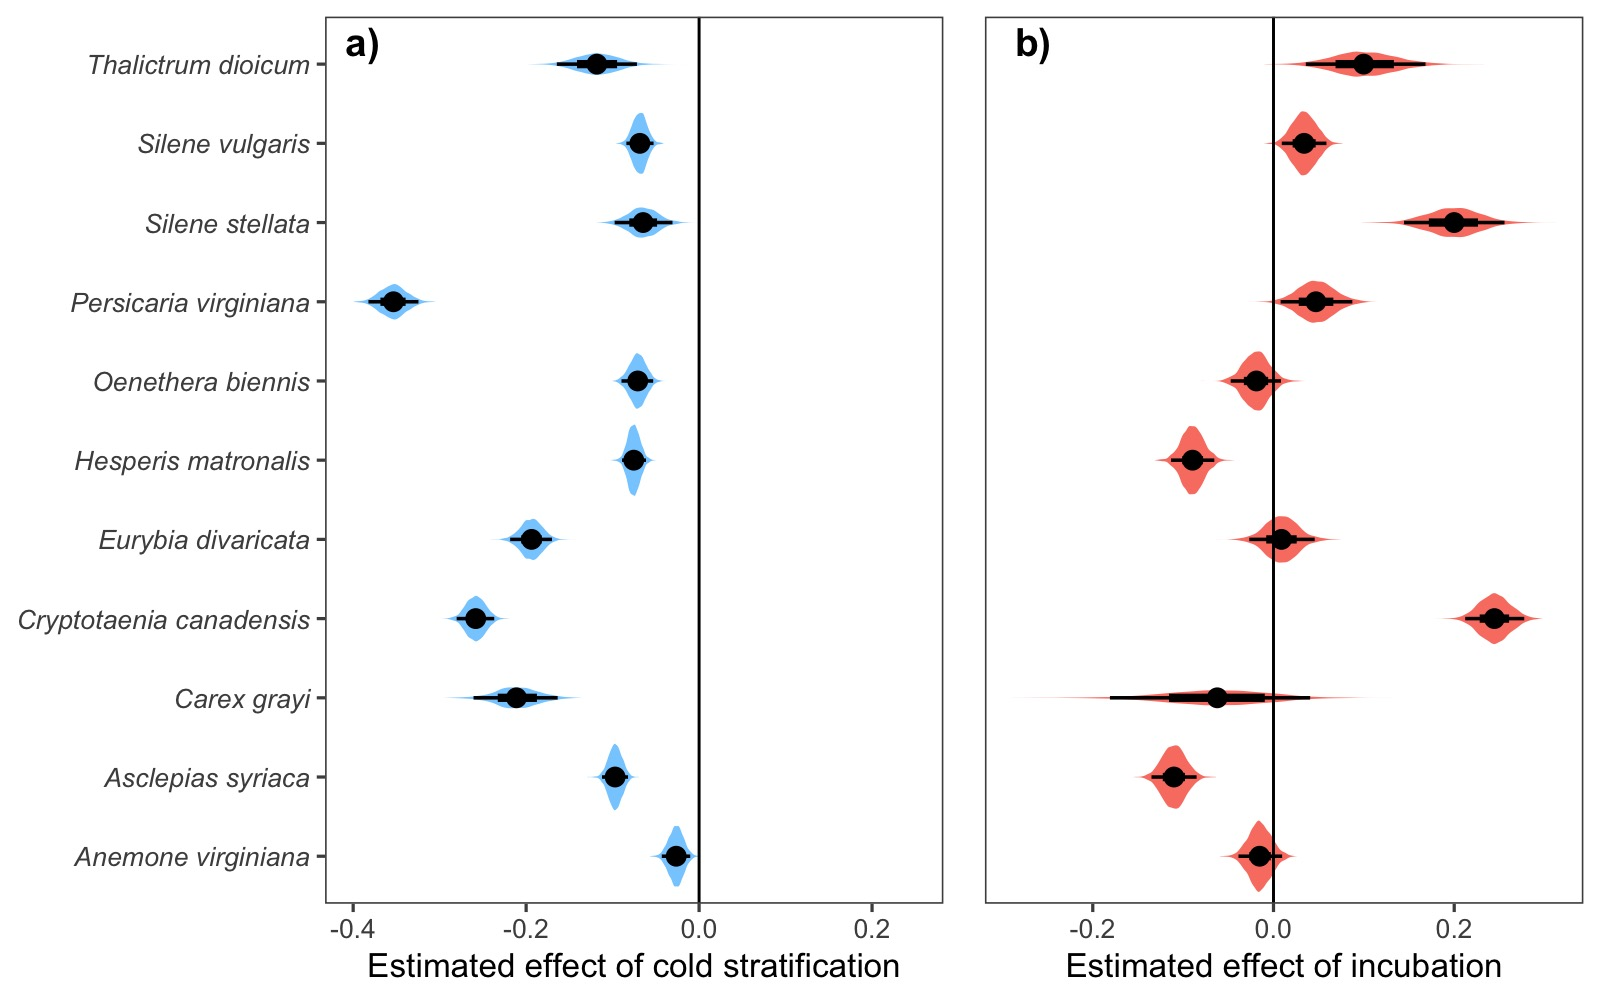
\includegraphics[width=\textwidth]{..//figure/mus_survival.jpeg}
   \caption{Estimated effects of weeks of cold stratification (\texitbf{a)} and incubation temperature (\texitbf{b)} on the time to 50\% germination (t50) for a suite of temperate herbaceous species. Negative estimates describe an advance in t50 and positive values a delay, estimates are on the log scale. The points indicate the mean estimated effect of each parameter, bars the  90\% uncertainty intervals, along with the full posterior distribution for each parameter as a full measure of uncertainty.} 
   \label{fig:musurv}
\end{figure}


\begin{figure}[h!]
    \centering
         %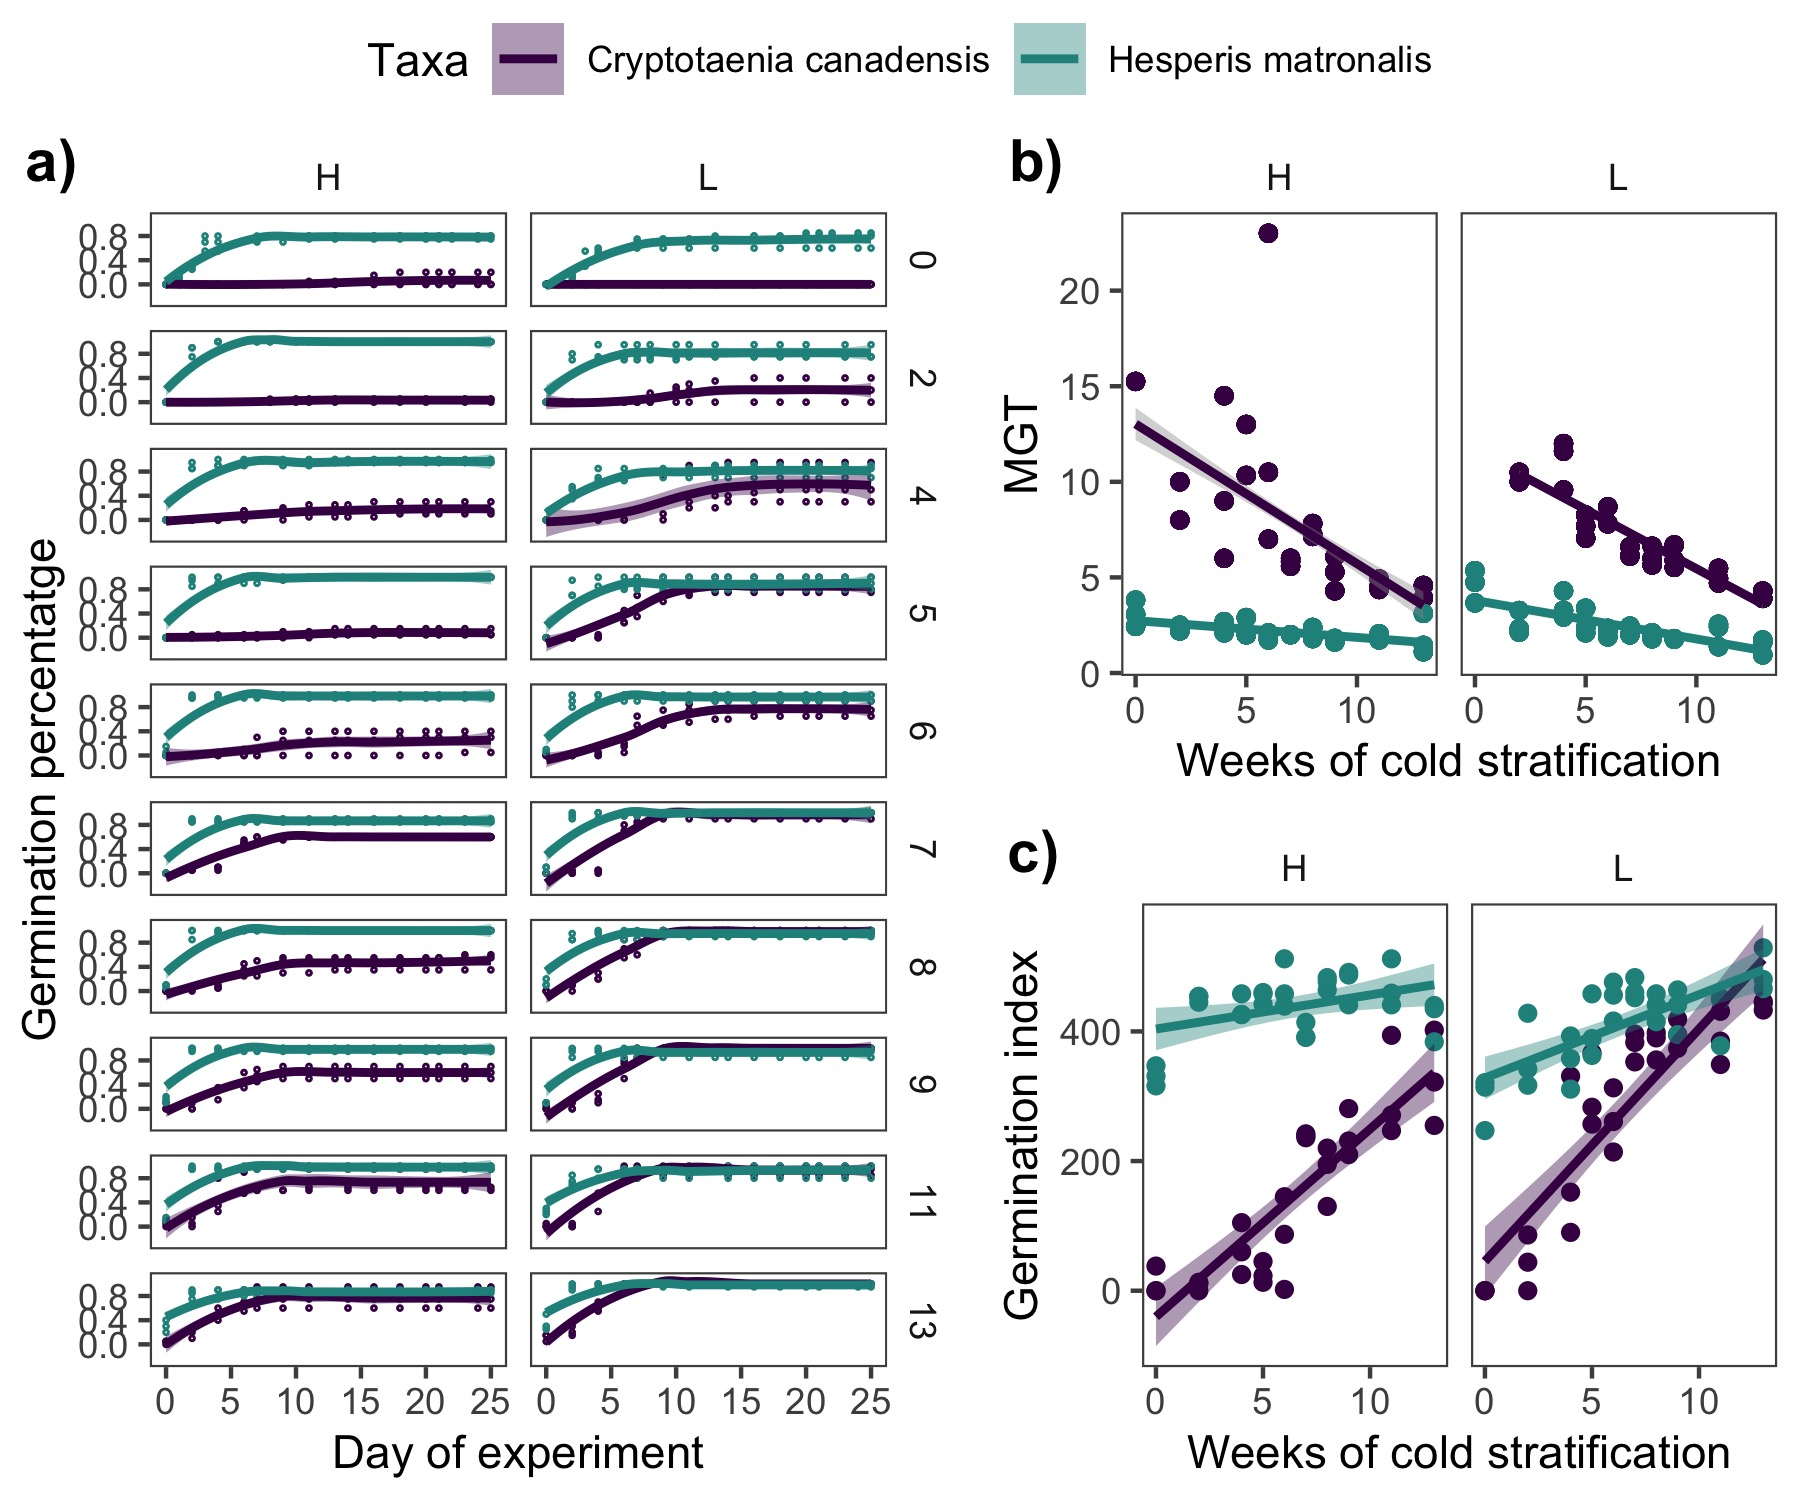
\includegraphics[width=\textwidth]{..//figure/crp_hesp1.jpeg}
          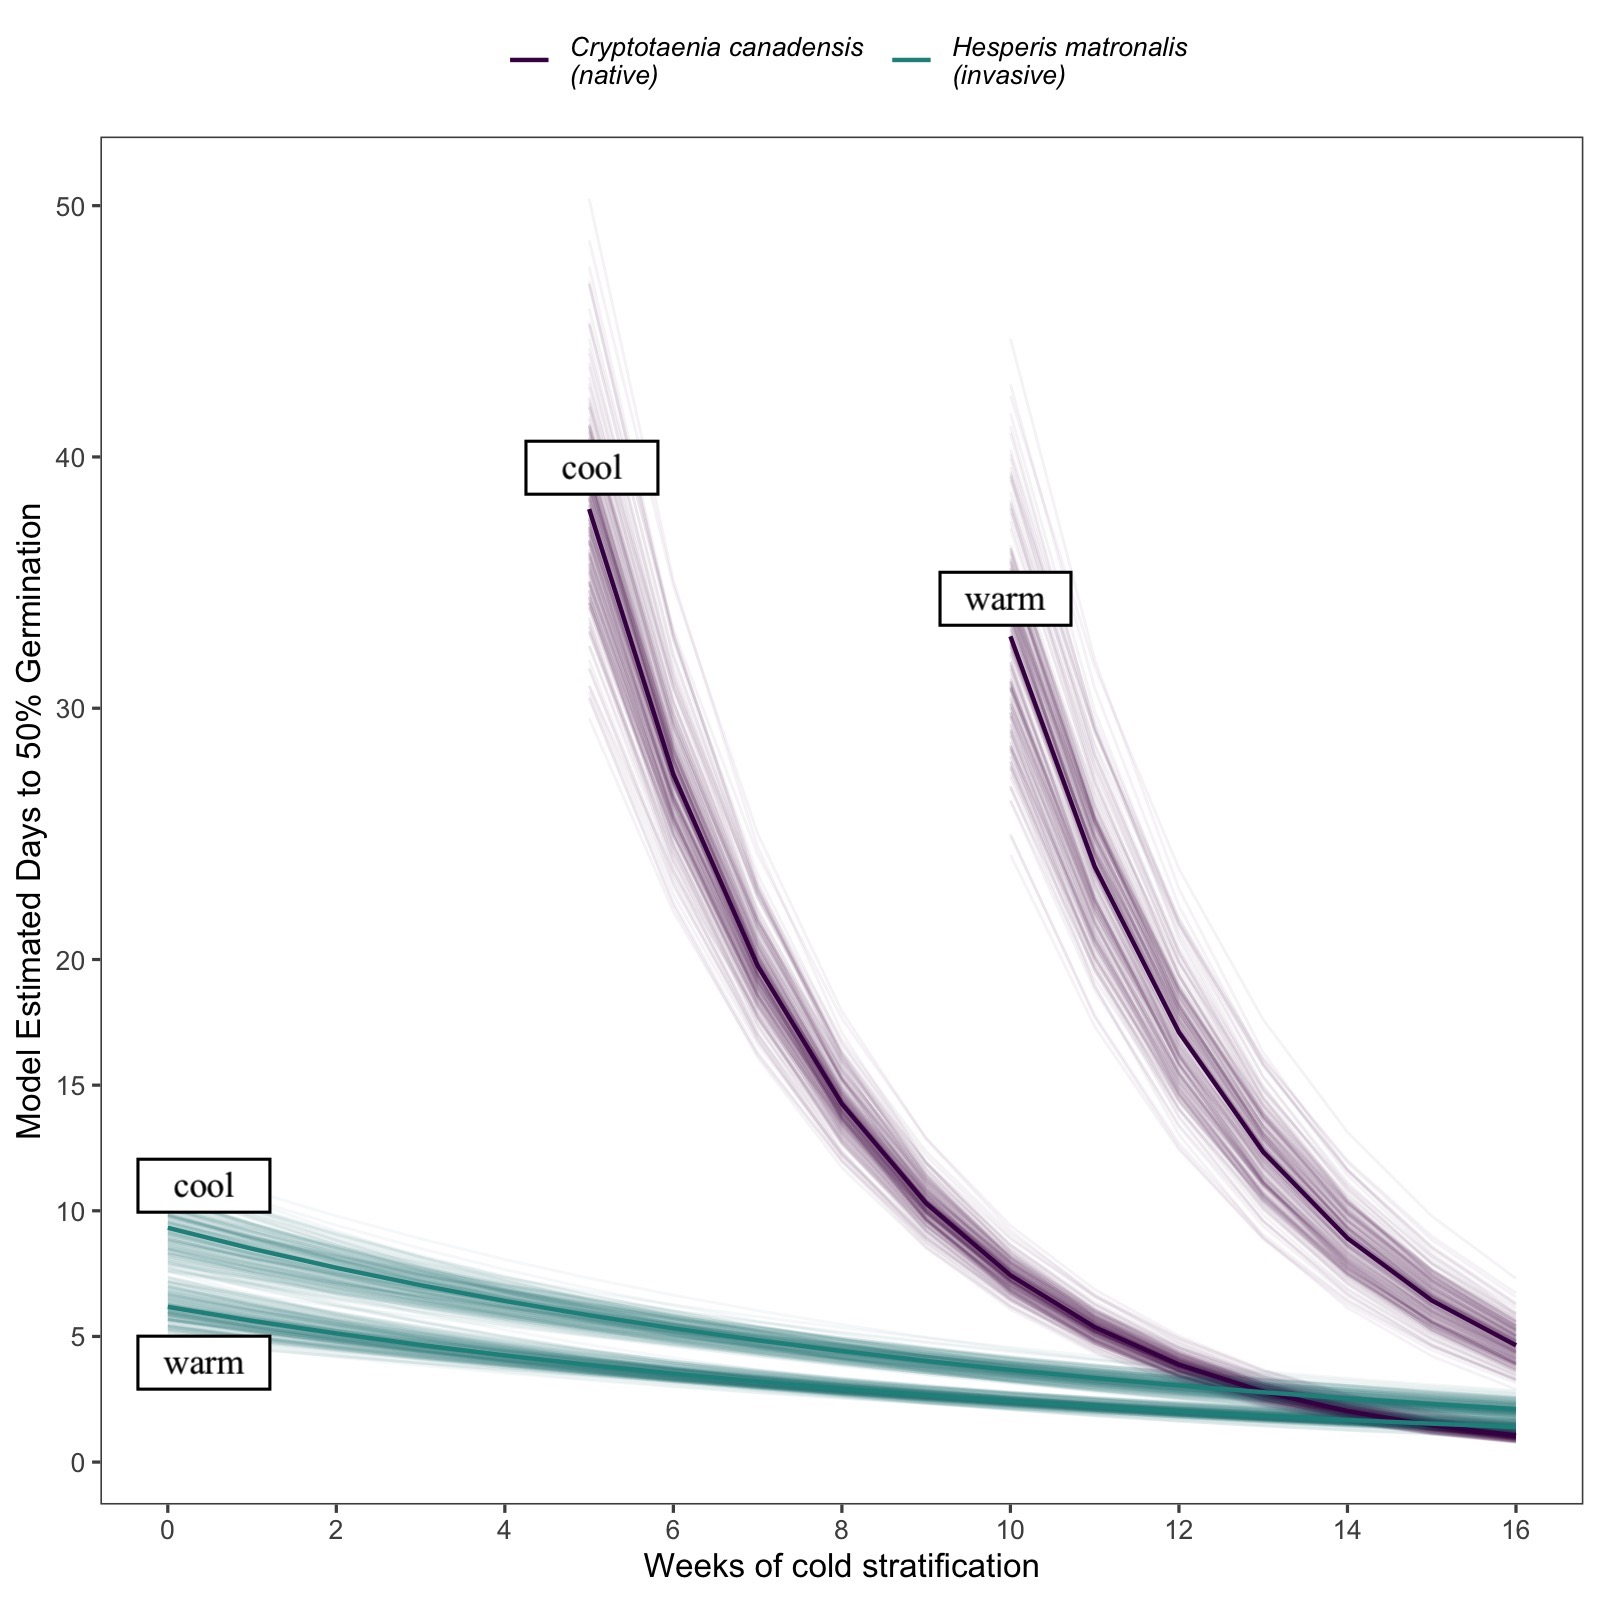
\includegraphics[width=\textwidth]{..//figure/AFTsivansive.jpeg}
%    \caption{Germination behavior of \textit{H. matronalis} and \texit{C. canadensis} indicate that the rate of \texit{C. canadensis} approaches that of \textit{H. matronalis} under cool temperatures and high levels of stratification. a) Shows germination time courses for both species at each level of incubation (H,L) and stratitification (0-13, y-axis). b) Dipicts Mean germination time for each species as a function of weeks of stratifcation and both high (H) and low (L) incubation temperature. c) Show a composite germination index for each species that account for the speed and percentage of germination for each species as a function of weeks of stratifcation and both high (H) and low (L) incubation temperature. } 
\caption{The effects of weeks of cold stratification at 4$^{\circ}$ C on the time to 50\% germination of \textit {Cryptotaenia canadensis} and \textit{Hesperis matronalis} under a) warm (20/10$^{\circ}$ C day/night) and b) cool (25/15$^{\circ}$ C day/night) incubation conditions, estimated with accelerated failure time model. Only stratification treatment levels which allowed both species to reach 50\% germination in less that 40 days are depicted here. The solid lines indicated indicated the mean estimate, while lighter line depict uncertainty.} %with 100 random draws from the posterior distribution.}
    \label{fig:aft}
\end{figure}


\begin{figure}[h!]
    \centering
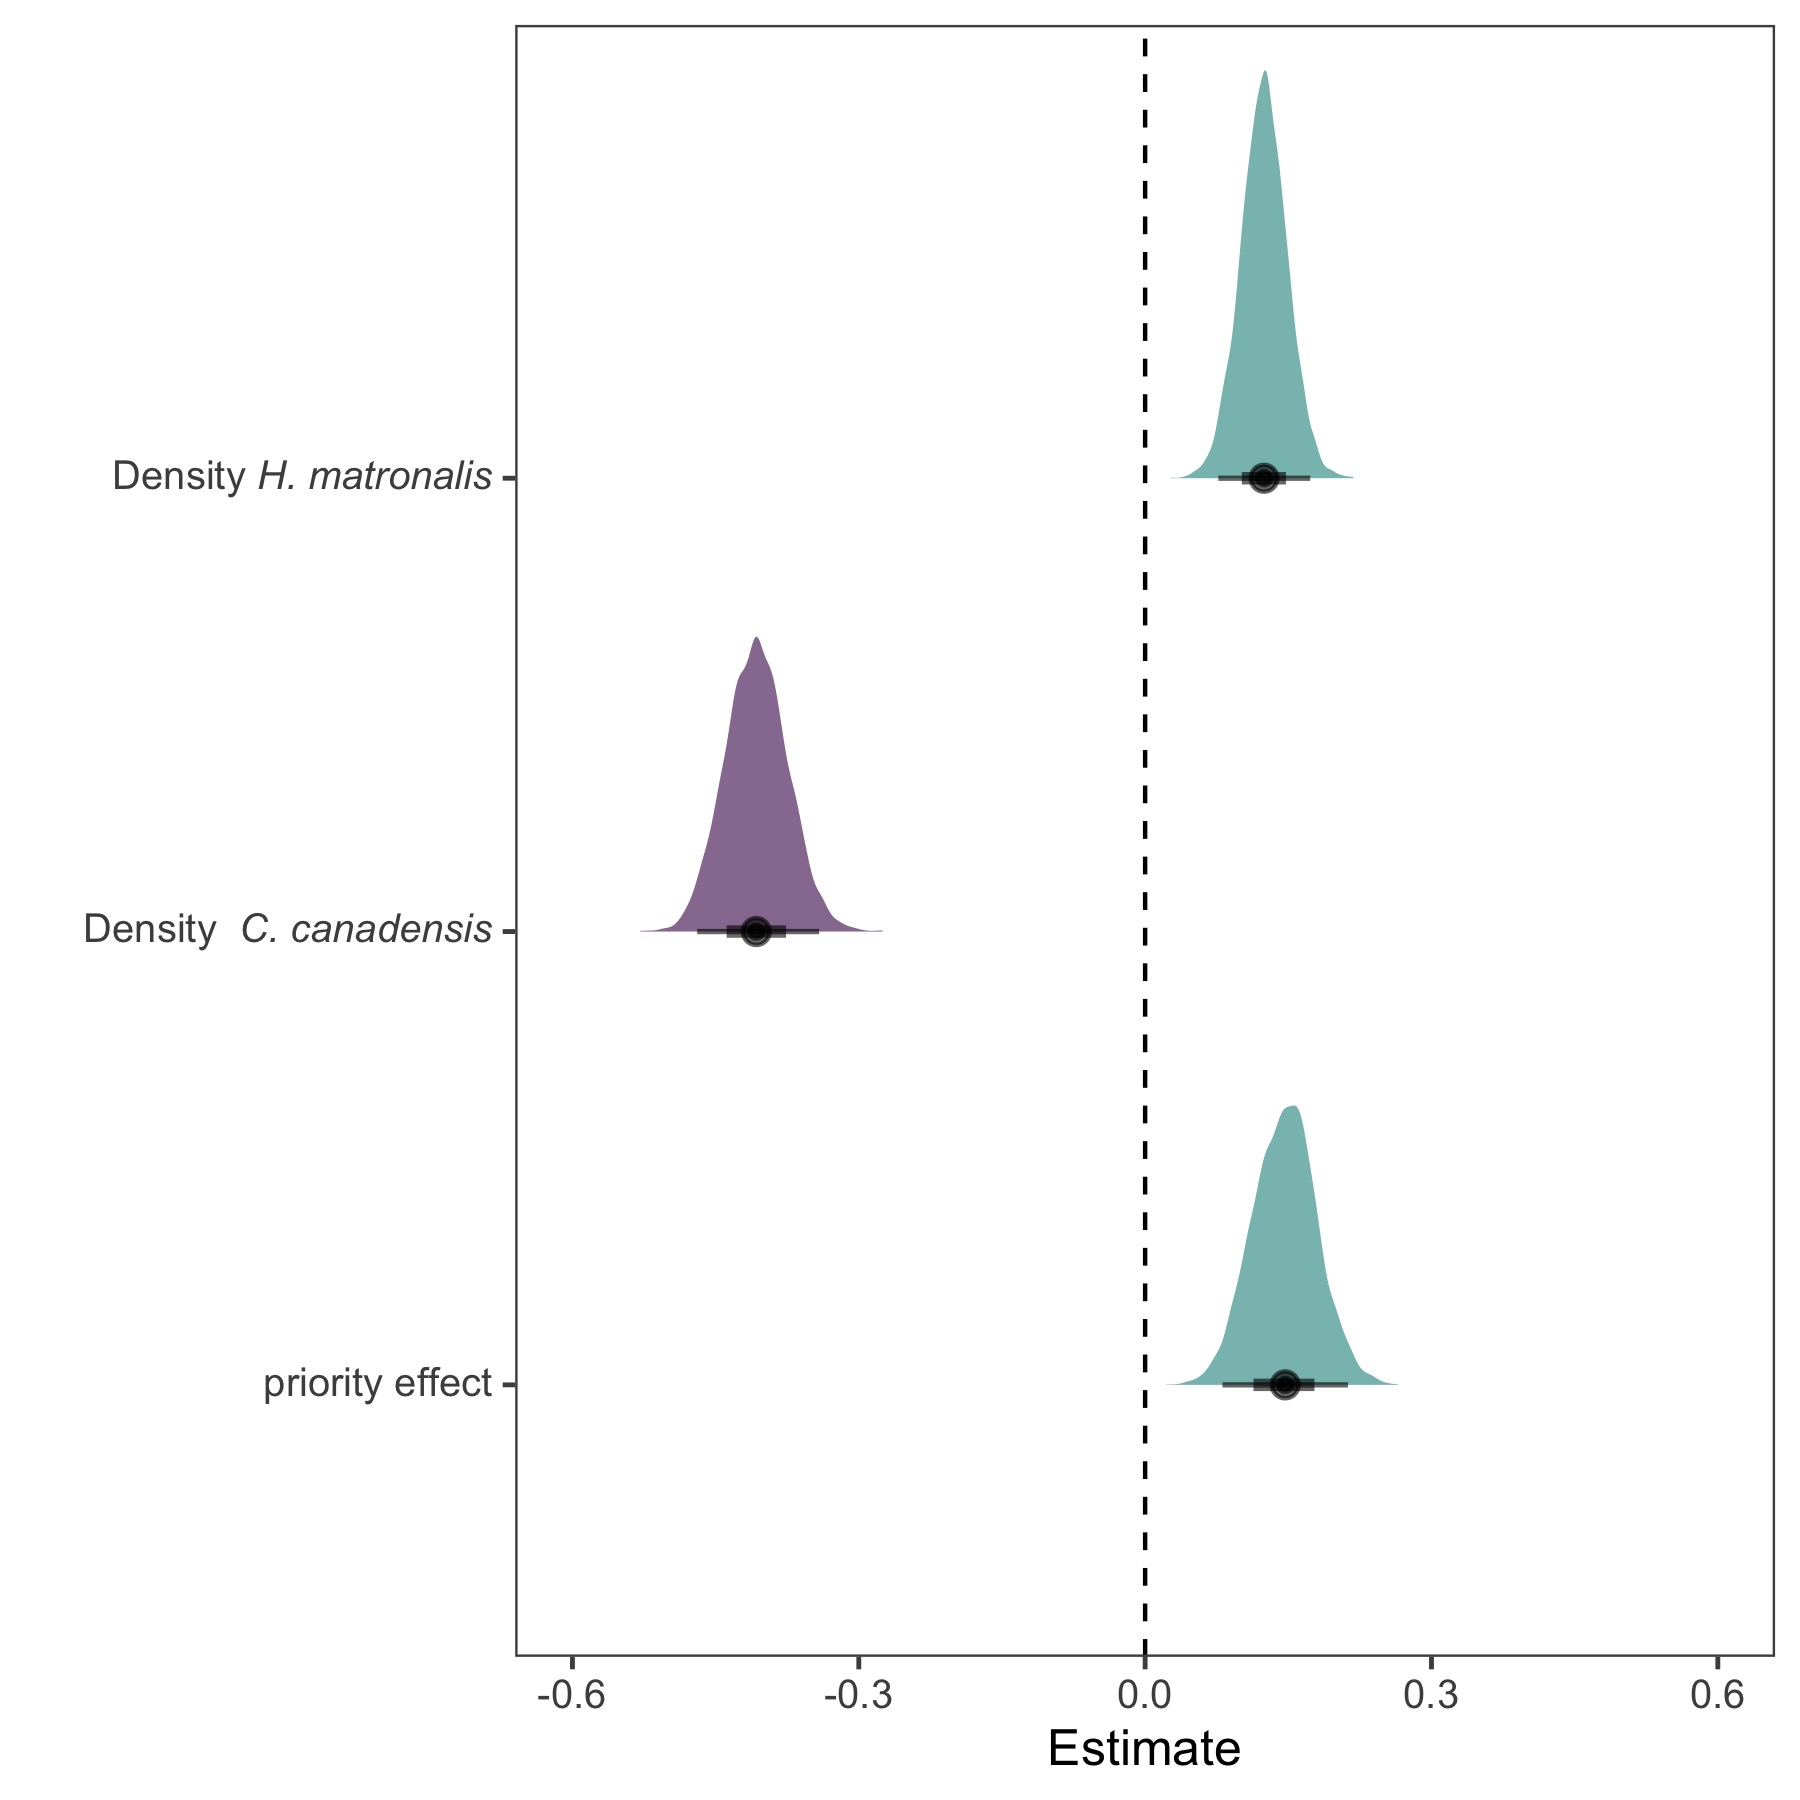
\includegraphics[width=\textwidth]{..//figure/mu_plots.jpeg}
    \caption{Estimated effects of species' abundance (species influence parameters) and phenological advantage (priority effects) on the relative growth rate difference between \textit{H. matronalis} and \textit{C. canadensis}. Negative parameter estimates indicate the community biomass composition shifts to favor \textit{C. candensis} while positive estimate towards dominance by \textit{ H. matronalis}. The points indicate the mean estimated effect of each parameter and bars the 90\% uncertainty intervals. The full posterior distribution for each parameter is also depicted as an additional measure of uncertainty.} 
    \label{fig:RGRD}
\end{figure}

\begin{figure}[h!]
    \centering
\includegraphics[width=\textwidth]{..//figure/3dconnolly2.png}
   \caption{Predicted outcome of competition under differing combinations of \textit{C. canadensis} and \textit{H. matronalis} abundance and phenological advantage of \textit{H. matronalis}. Purple dots indicate conditions that favor  \texit{C. canadensis} in community biomass composition while green dot conditions favor \textit{H. matronalis}. Estimates are based on multiple regression models estimating the effect of each variable on the relative growth rate difference among species.} 
   \label{fig:3D}
\end{figure}

\begin{figure}[h!]
    \centering
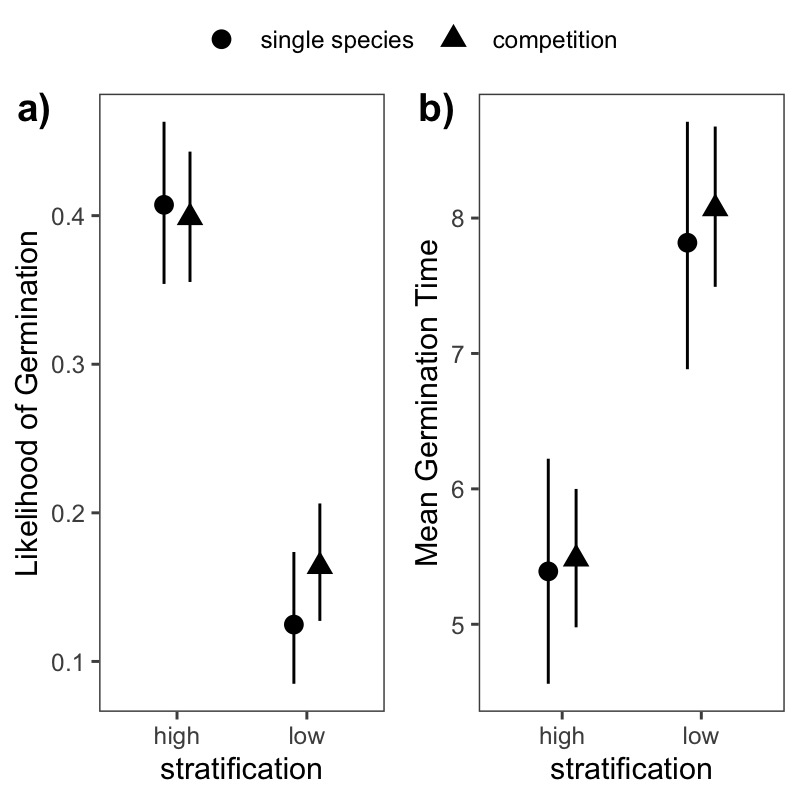
\includegraphics[width=.7\textwidth]{..//figure/nichemodfication.jpeg}
   \caption{Estimated effects of intra-vs. inter-specific competition on the germination dynamics of \textit{Cryptotania canadensis} under 6 (low) and 10 weeks (high) of cold stratification at 4$^{\circ}$C. Panel \textbf{a)} depicts differences germination likelihood and \textbf{b)} shows the estimated mean germination time in single species mono-cultures vs. competition plot. Colored dots represent the mean estimate under each planting type and bars represent 90\% uncertainty intervals. } 
   \label{fig:nichemod}
\end{figure}

\begin{figure}[h!]
    \centering
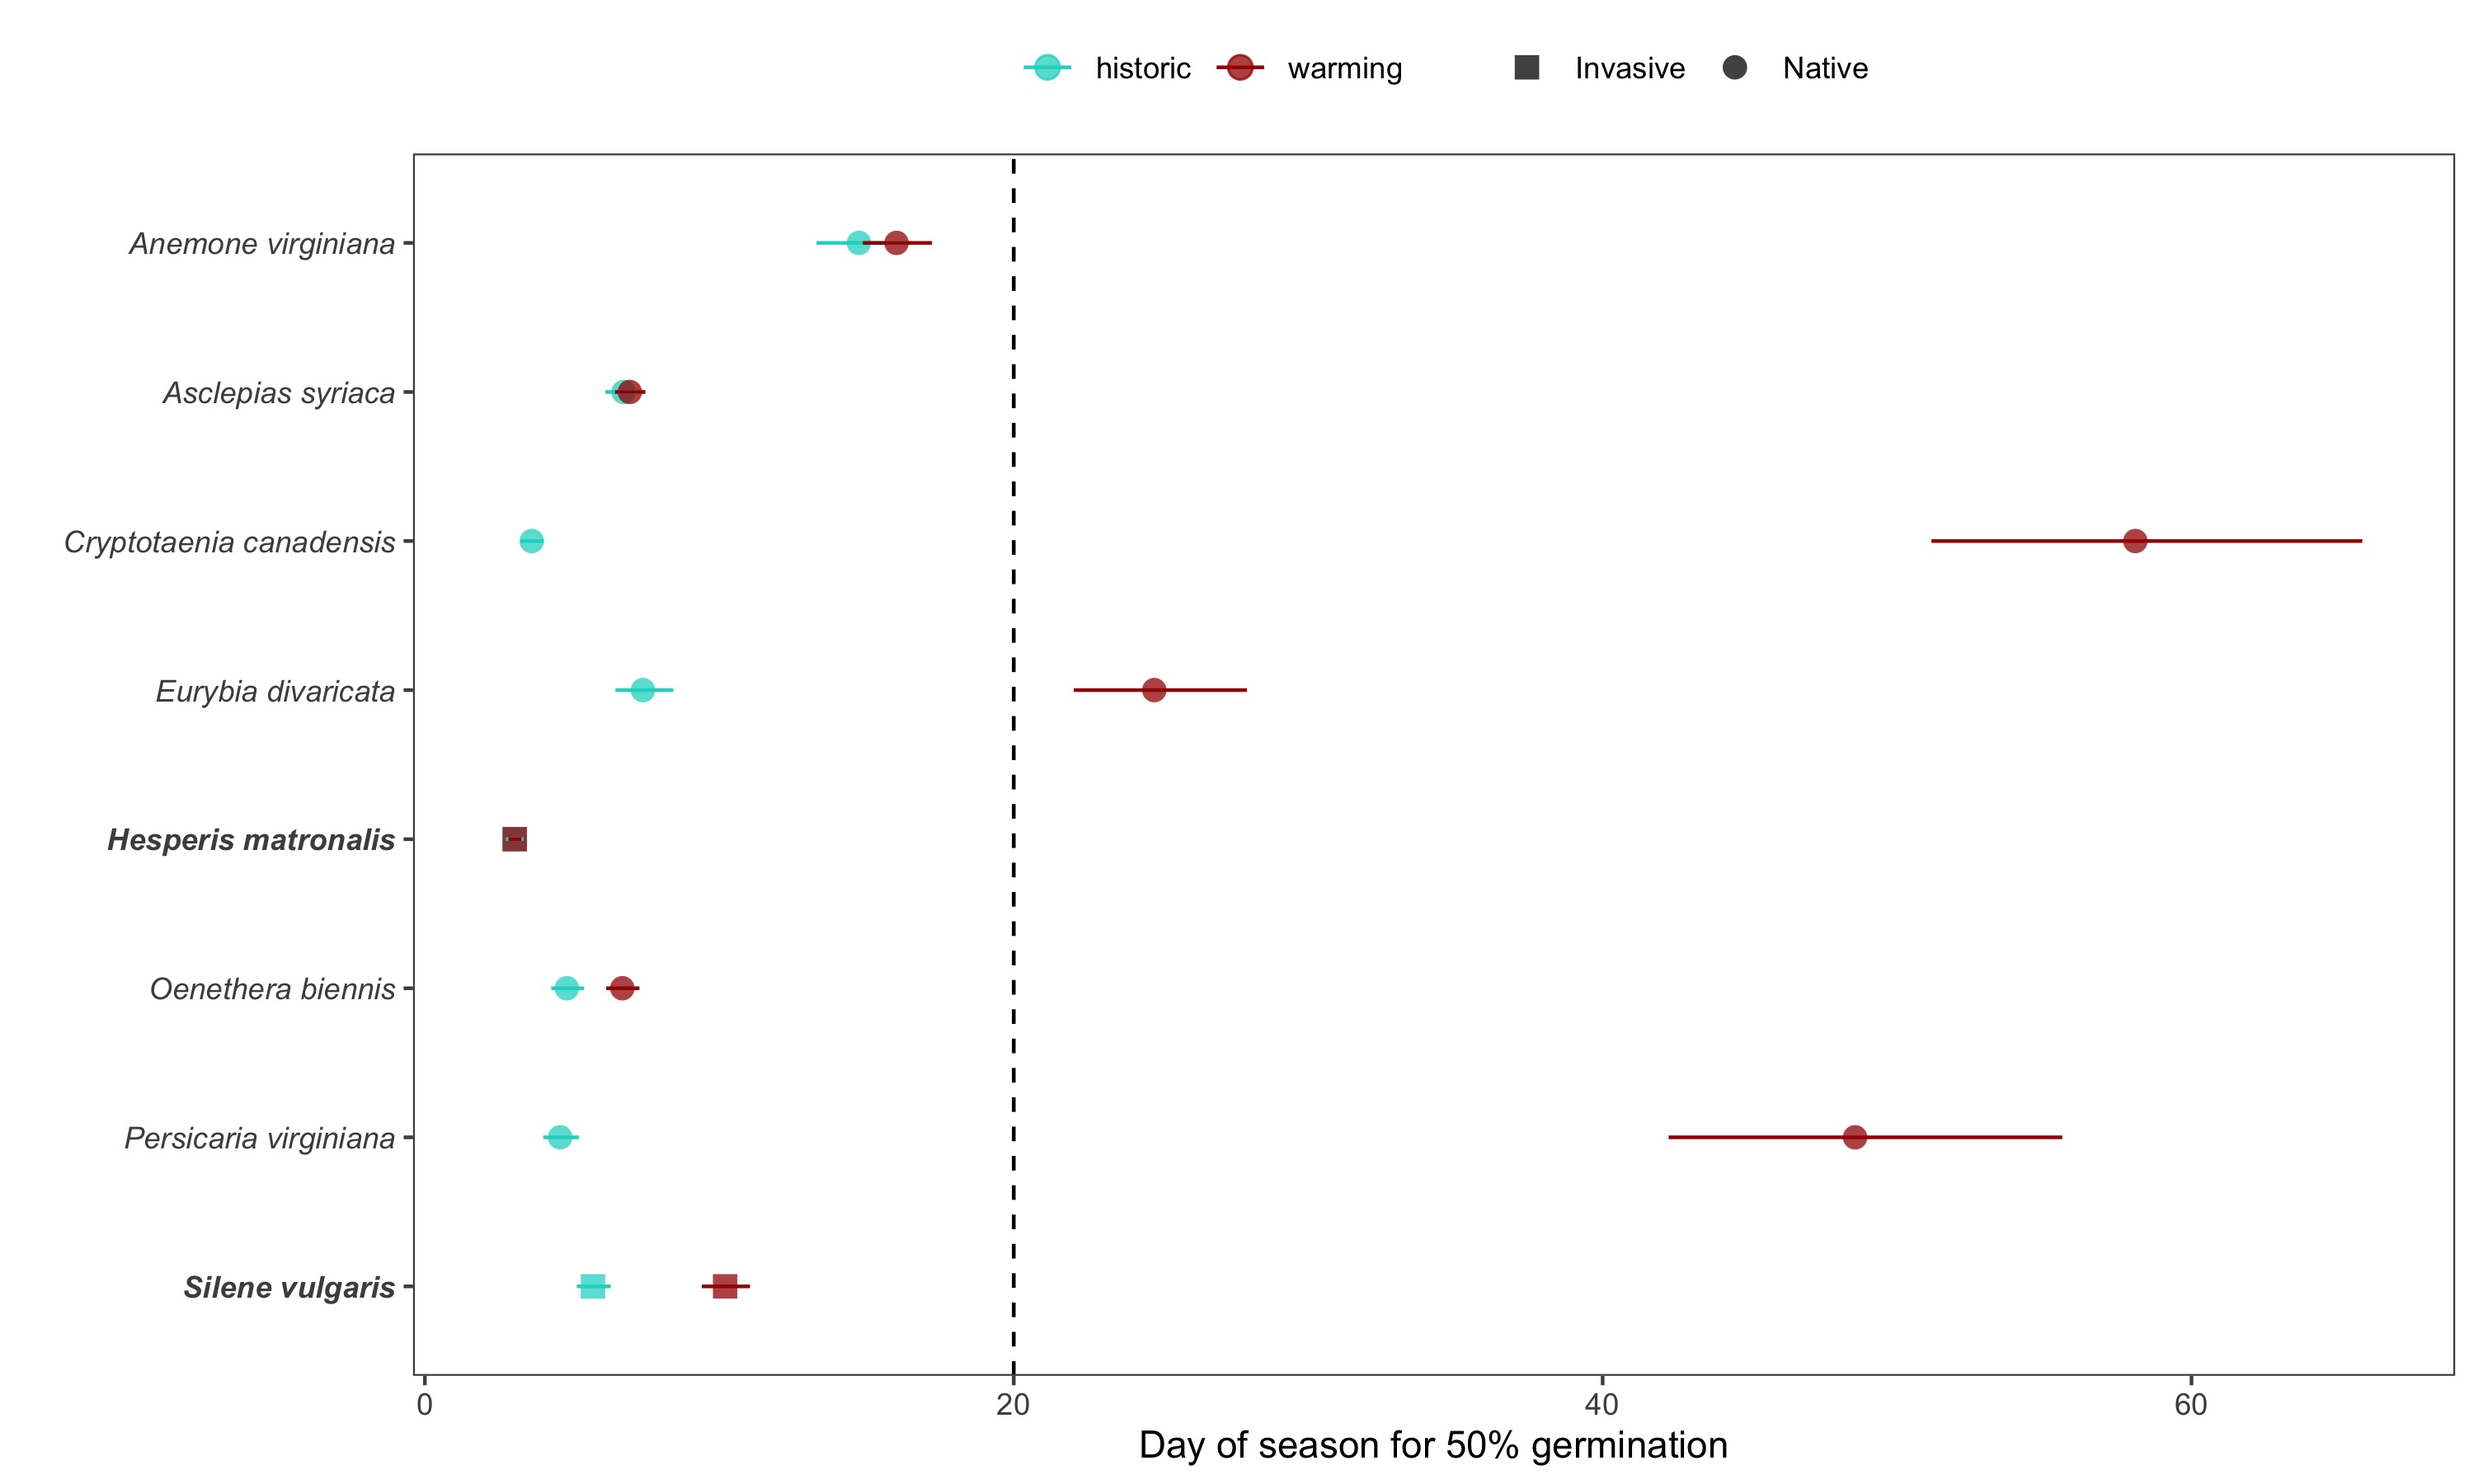
\includegraphics[width=\textwidth]{..//figure/commchange.jpeg}
   \caption{Predicted germination phenology of a suite of temperate herbs under historic (10 weeks cold stratification at 4$^{\circ}$ C and  20/10$^{\circ}$ incubation)  and climate warming scenarios (10 weeks cold stratification at 4$^{\circ}$ C and  20/10$^{\circ}$ incubation).  Warming reduces the ratio of native to invasive species that germinate within 20 days of the growing period, and increases the phenological advantage of the invasive species in this study. Points represent mean estimates of time to 50\% germination and bars represent 90\% uncertainty intervals } 
   \label{fig:comm}
\end{figure}



%In combination our germination assays,The germination behavior of \texit{H. matronalis} was little affected by cold stratification, while germination rate and speed of \texit{C. canadensis} was strongly enhanced with cold stratification, especially when germianted at cooler temperatures (Fig. \ref{fig:aft}). These differences are themselves not surprising as \textit{H. matronalis} seeds are considered non-dormant \citep{}, and seeds of \textit{C. canadensis} are physiologically dormant \citep{}. , These different responses generated germination dynamics in which under alternative low stratification regimes \textit{H. matronalis} cohorts germinated as much as two weeks before \textit{C. canadensis}, while under high stratification, the species germinated at approximately the same time (Fig. \ref{fig:aft}). 

%In our competition trials, we observed that differences in germination on the order of a few days had substantial impacts on both the per capita and plot level relative growth rate differences among species (Fig \ref{fig:Cc},\ref{fig:RGRD}). If we consider the range of variability we observed (approximately two weeks lag to simultaneously)

%These inter-specific dynamics we observed are comparable to treatments applied in staggered planting experiments \citep{}, but the fact that we were able to induce these effects through varying the germination environment rather than directly manipulating germination itself is an important phase for translating the estimates from priority effect experiments into natural systems.  suggests that the kinds of seasonal priority effects may be important for realz, especially in seasonal environments with high levels of inte-rannual climate variations.



\end{document}

%\noindent We assessed the impact of competitor density and relative germination timing on species biomass with two different frameworks.

%First we calculated the average per-capita biomass of each species per pot, by divided each species' plot level biomass by its number of germinants. We then set up a system of pair-wise equations in which the per-capita biomass of each species was regressed against the density of con-specific seeds, density of competitor seeds, and the difference in mean germination time among them using Bayesian linear models. The equation is written below.
%
%\begin{align*}

%biomass_{C. canadensis}  &= \alpha +& \beta_{1}*density_{C. canadensis} + \beta_{2}*density_{H. matronalis}+\beta_{3}*$\delta$MGT + \epsilon} 

%biomass_{H. matronalis}  &= \alpha +& \beta_{1}*density_{C. canadensis} + \beta_{2}*density_{H. matronalis}+\beta_{3}*$\delta$MGT + \epsilon}

%\end{align*}

%
%In the formulation, the $beta$_1$ is the estimated effect of intra-specific competition, $beta_2$ is the estimated effect of inter-specific competition, and $beta_3$ is the estimated priority effect. From these estimates we calculated the competition coefficients (c) (ratio of intra- to inter-specific competition strength) for each species, with and without the additive effects of germination phenology differences.

%\begin{align*}
%
%$c_{sp1} $ &= $ \frac{b_{1}}{b_{2}} $

%$c_{prioritysp1}$ &= $\frac{(b_1+b_3)}{b_2}$

%\end{align*}
